%% apendice-fase-previa.tex — La fase previa: prueba de la hipótesis confuciana
\chapter{La Fase Previa: Prueba Semántica de la Hipótesis Confuciana}
\label{anexo:fase-previa}

Este anexo documenta la fase anterior de esta investigación, citada a lo largo de los capítulos como antecedente directo de la pregunta del eco y la voz. En esa fase, el mismo corpus de nueve unidades se analizó bajo una pregunta distinta: ¿la herencia educativa confuciana predice convergencias semánticas entre las políticas de IA del Sudeste Asiático, tomando a China como caso ancla de esa tradición? La hipótesis se operacionalizó como una expectativa de agrupamiento verificable: si la herencia confuciana pesa en el discurso, los países de herencia fuerte (Vietnam, Singapur) deberían presentar mayor similitud entre sí y con China que con sus vecinos no confucianos.

\section{Matriz de Similitud}

La Tabla~\ref{tab:anexo-similitud} reproduce la matriz de similitud coseno entre los centroides de los nueve documentos (modelo multilingüe local, 2{,}334 fragmentos), y la Figura~\ref{fig:anexo-heatmap} su mapa de calor.

\begin{table}[htbp]
\centering
\caption{Matriz de similitud semántica entre las nueve unidades del corpus (fase previa)}
\label{tab:anexo-similitud}
\footnotesize
\begin{tabular}{lccccccccc}
\hline
 & \textbf{Chi} & \textbf{Vie} & \textbf{Sin} & \textbf{Mal} & \textbf{Ind} & \textbf{Tai} & \textbf{Fil} & \textbf{ASE} & \textbf{UNE} \\
\hline
China      & 1.000 & 0.712 & 0.676 & 0.650 & 0.804 & 0.614 & 0.668 & 0.580 & 0.564 \\
Vietnam    & 0.712 & 1.000 & 0.896 & 0.909 & 0.809 & 0.830 & 0.850 & 0.851 & 0.719 \\
Singapur   & 0.676 & 0.896 & 1.000 & 0.948 & 0.769 & 0.841 & 0.887 & 0.871 & 0.722 \\
Malasia    & 0.650 & 0.909 & 0.948 & 1.000 & 0.784 & 0.892 & 0.914 & 0.874 & 0.729 \\
Indonesia  & 0.804 & 0.809 & 0.769 & 0.784 & 1.000 & 0.760 & 0.807 & 0.755 & 0.742 \\
Tailandia  & 0.614 & 0.830 & 0.841 & 0.892 & 0.760 & 1.000 & 0.861 & 0.777 & 0.667 \\
Filipinas  & 0.668 & 0.850 & 0.887 & 0.914 & 0.807 & 0.861 & 1.000 & 0.813 & 0.724 \\
ASEAN      & 0.580 & 0.851 & 0.871 & 0.874 & 0.755 & 0.777 & 0.813 & 1.000 & 0.770 \\
UNESCO     & 0.564 & 0.719 & 0.722 & 0.729 & 0.742 & 0.667 & 0.724 & 0.770 & 1.000 \\
\hline
\end{tabular}
\end{table}

\begin{figure}[htbp]
\centering
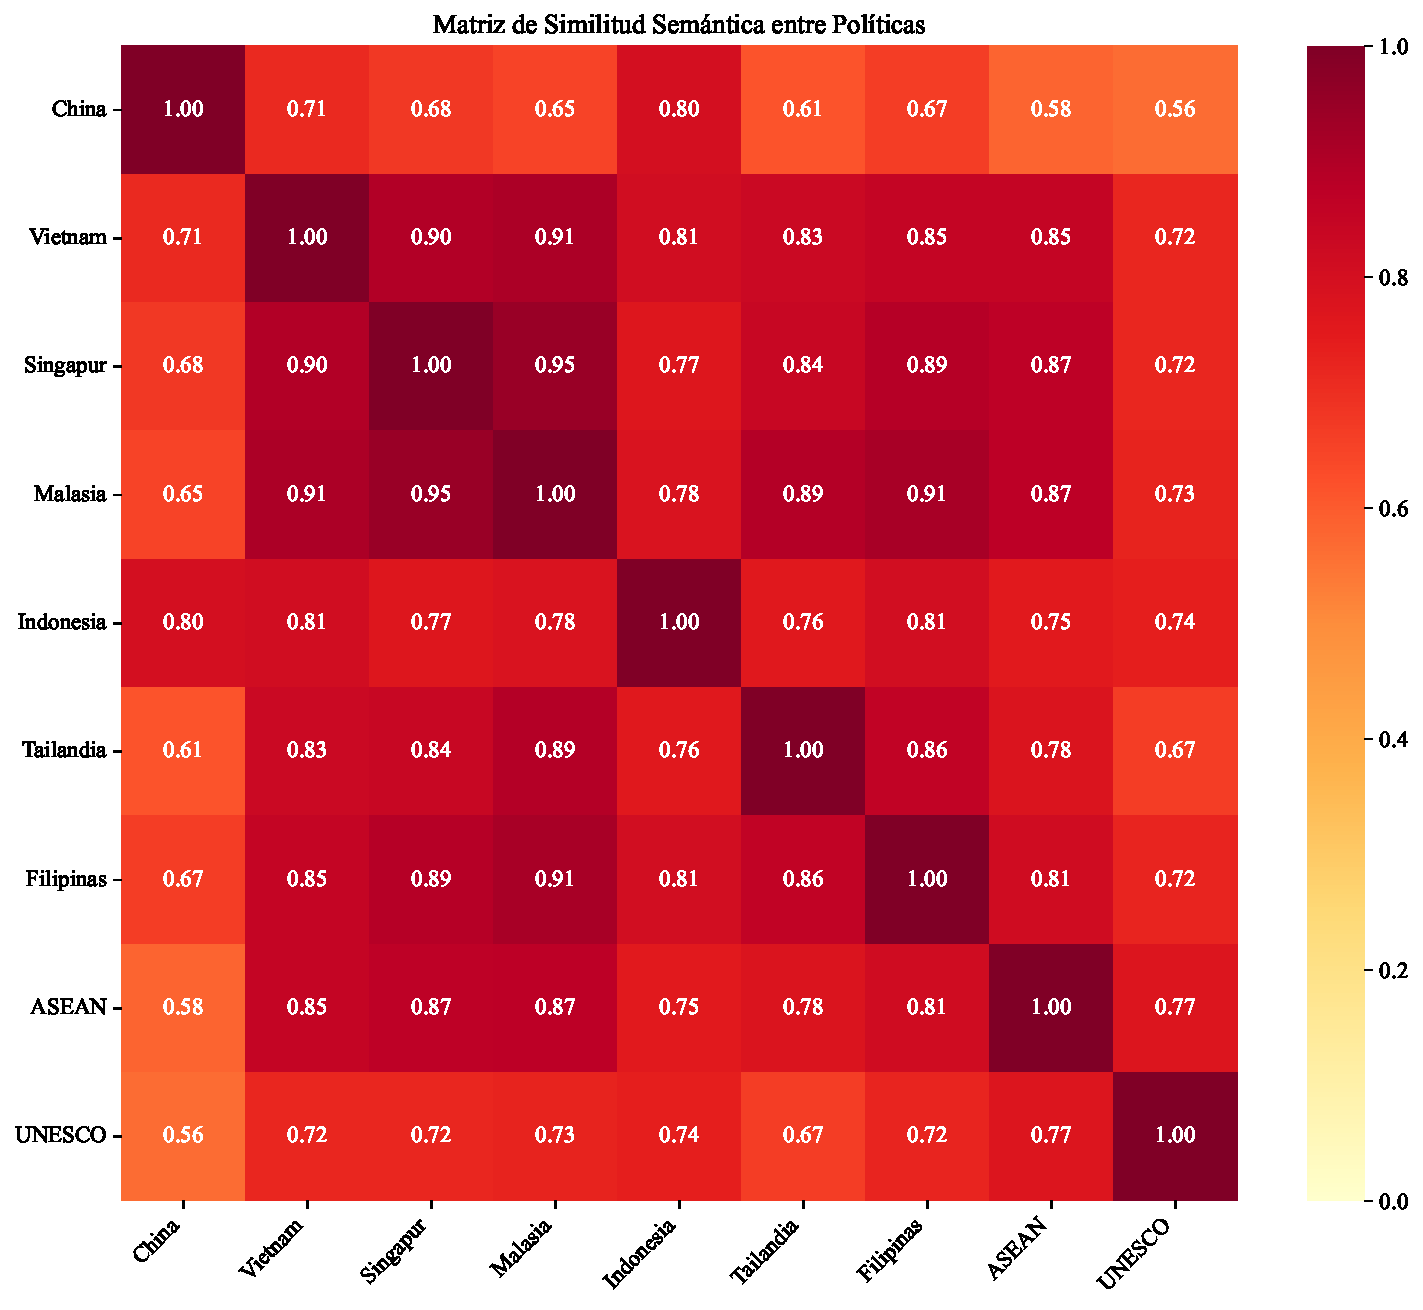
\includegraphics[width=\textwidth]{figures/generated/heatmap_similitud.pdf}
\caption{Mapa de calor de la matriz de similitud semántica (fase previa).}
\label{fig:anexo-heatmap}
\end{figure}

\section{Agrupamiento Jerárquico y Resultado de la Prueba}

El agrupamiento jerárquico (método de Ward sobre la matriz de distancias) produce una estructura estable de tres grupos en un rango amplio de umbrales de corte (0.196 a 0.347). El orden de fusión es el dato central: Singapur y Malasia se unen primero (distancia 0.052), después Vietnam (0.109), Filipinas (0.133), Tailandia (0.166) y la ASEAN (0.191); China e Indonesia forman un segundo grupo (0.196); y la UNESCO permanece aislada hasta el final de la jerarquía (0.347).

La hipótesis confuciana no se sostuvo en ninguno de sus dos componentes. En el componente horizontal, la similitud Vietnam--Singapur (0.896) es alta pero no distintiva: queda por debajo de pares que cruzan la frontera cultural (Singapur--Malasia, 0.948; Malasia--Filipinas, 0.914), y ningún corte del dendrograma produce un grupo \{Vietnam, Singapur\} ni \{China, Vietnam, Singapur\}. En el componente vertical, el caso ancla no atrae a sus herederos culturales: el par más próximo de China es Indonesia (0.804) —país sin herencia confuciana, pero con el mismo género documental de planificación integral de largo horizonte—. El espacio semántico se organiza por género y escala documental (los dos documentos mayores del corpus se agrupan entre sí) y por pertenencia regional (las cinco estrategias nacionales con la guía ASEAN), no por matriz cultural.

\section{De la Fase Previa a esta Tesis}

El resultado negativo, leído junto con la literatura crítica del constructo de Culturas de Herencia Confuciana~\citep{ryan2007false, odwyer2017deflating}, motivó la reformulación que estructura esta tesis: si las políticas no se agrupan por sus tradiciones, la pregunta productiva no es si la cultura causa el discurso, sino qué calidad tiene aquello en lo que las políticas convergen (la evaluación con rúbrica) y si en esa convergencia sobrevive alguna voz local (el índice de voz y la validación literal). La triangulación de aquella fase dejó además la fórmula que esta tesis somete a verificación evaluativa: las huellas de la tradición detectables cualitativamente residen en la forma institucional de las políticas —la verticalidad del decreto, el plan integral, la meta clasificatoria—, no en su vocabulario. Los capítulos~\ref{cap:resultados} y las conclusiones retoman ambos hilos con los instrumentos de esta fase.
